{
\chapter{Background}
\label{ch:background}
\renewcommand{\chapterpath}{includes/background}
The purpose of this chapter is two-fold: First, it aims at providing the fundamental background about the most relevant aspects of machine learning for this thesis, such as the theory of generalisation and regularisation. Second, it is also intended to serve as a review of the relevant and related scientific literature.

The introduction to the core aspects of machine learning in this chapter is deliberately non-exhaustive, as it is intended to provide only a sufficient background to enable the understanding of the rest of the thesis to a wider audience. The interested reader may follow the references to scientific literature provided throughout the chapter.

\section{Machine learning fundamentals}
Humans perceive the world and make sense of it in a great variety of ways: we see light as visual information, hear sounds and create music, use language to produce written text and speech and organise much of what we know into collections of numbers, to name a few. As diverse as light, sound, language and numbers are, they can all be conceptualised as \textit{data}. Thinking of what we perceive and know about the world as information that can be organised into data is a powerful formal conceptualisation that allows us to better understand and analyse the input and output we perceive and generate.

Machine learning is the discipline that studies how to automatically discover patterns from data \citep{murphy2012machinelearning}. Much as humans and other animals are able to make sense of the world out of what they perceive, machine learning aims at providing the methods to make sense out of formally defined data points, that is learning from data \citep{abu2012learningfromdata}. Machine learning has its roots in mathematics and statistical inference, but has developed as a distinct field after the development and spread of computers and computer science, which have provided the means to store and process data efficiently and automatically. 

\subsection{Elements of machine learning}
\label{sec:background-elements_ml}
The fundamental component of machine learning is the data and, as motivated above, the field itself arises from the ability to map any observation of the world into data points. Formally, one can define one data point as an $M$-dimensional vector $\mathbf{x} = x_{j}, \ldots, x_{M}$. Then, a set of $N$ observations $\{\mathbf{x}_{i}\}_{i}^{N} \in \mathcal{X}$ is said to be the \textit{input} data set. Most of the machine learning literature \citep{alpaydin2009machinelearning, abu2012learningfromdata, murphy2012machinelearning} makes a broad distinction amongst machine learning methods depending on the \textit{output} or \textit{target} data. A non-exhaustive taxonomy of the main types of machine learning methods as commonly found in the literature is the following:

\begin{itemize}
  \item \textbf{Supervised learning}: in a supervised learning setting, every observation $\mathbf{x}_{i}$ is paired with an output variable $y_{i}$, also referred to as \textit{ground truth}, and thus the data set is considered $\mathcal{D} = \{(\mathbf{x}_{i}, y_{i})\}_{i}^{N}$. The goal of supervised learning is discovering the relationship between the input data $\mathbf{x}_{i}$ and the target variables $y_{i}$. Depending on the nature of $y_{i}$, the learning problem can be \textit{classification} or \textit{regression}:
  \begin{itemize}
    \item Classification: $y_{i} \in \{1, \ldots, C\}$ is a discrete or categorical value. The possible values of $y$ are also referred to as \textit{classes} or \textit{labels}.
    \item Regression: $y_{i} \in \mathbb{R}$ is a continuous variable.
  \end{itemize}
  \item \textbf{Unsupervised learning}: in an unsupervised learning setting, there is not explicit access to target variables. Therefore the data set is simply $\mathcal{D} = \{\mathbf{x}_{i}\}_{i}^{N}$, and the goal is to discover patterns in the input data. A prototypical example of unsupervised learning is clustering.
  \item \textbf{Reinforcement learning} is a broad class of machine learning methods, initially inspired by behavioural psychology and the concept of trial-and-error learning. Instead of a mapping between input and output variables, in reinforcement learning typically there is access to a \textit{reward} signal that might not be available for every input data point. The goal is to learn policy that maximises the expected rewards by seeking a balance between exploration and exploitation.
\end{itemize}

While this distinction is useful, the boundaries are sometimes blurred, in practice. For example, some problems often labelled as unsupervised learning could be considered particular cases of supervised learning, as we have discuss in the Introduction (Section~\ref{sec:intro-rethinking_supervised}). Most of the problems that we will address in this thesis can be defined within a supervised framework and, more specifically, classification. For these reasons, in the remaining of this section we will focus on classification, unless specified otherwise.

As introduced above, the goal of a (supervised) machine learning method is to discover the relationship between the input data and the target variables. This assumes that such relationship is determined by an underlying, unknown function $f \colon \mathcal{X} \mapsto \mathcal{Y}$. Since $f$ is a latent function, the task is to find a function $g \in \mathcal{H} \colon \mathcal{X} \mapsto \mathcal{Y}$ from a set of candidate functions $h \in \mathcal{H}$---the hypothesis set---that approximates $f$ according to certain error or loss measure $L(h, f)$. In order to find $g$, the \textit{learning algorithm} $\mathcal{A}$ uses the available \textit{training} data $\mathcal{D} = \{(\mathbf{x}_{i}, y_{i})\}_{i}^{N} = (\mathbf{x}_{1}, y_{1}), \ldots, (\mathbf{x}_{N}, y_{N})$ to solve an optimisation problem by adjusting a set of learnable parameters $\boldsymbol{\theta}$. Hence, the task is to determine from the set of functions $h(\mathbf{x}; \boldsymbol{\theta})$, the one which best approximates the data $\mathcal{D}$.

Nonetheless, if the relationships found apply only to the training data $\mathcal{D}$, then the process could not be considered \textit{learning}, but at best memorisation. Crucially, the ultimate objective of machine learning is to learn relationships and make correct predictions beyond the observed data. This is called \textit{generalisation}. This notion of learning is only feasible in a probabilistic way. The probabilistic view introduces the important assumption that the relationship between the targets $y$ and the input $\mathbf{x}$ is not deterministic, but probabilistic and there exists an unknown, underlying joint probability distribution $P_{X,Y}(\mathbf{x}, y)$ on $\mathcal{X} \times \mathcal{Y}$---thus also a marginal input distribution $P_{X}(\mathbf{x})$ and a conditional output distribution $P_{Y|X}(y|\mathbf{x})$, in Bayesian terms. Furthermore, it is also generally assumed that the observed available data points were sampled independently from $P_{X,Y}$. A summary schematic of the main elements of supervised learning is shown in Figure~\ref{fig:background-elements_learning}.

\begin{figure}[htb]
  \begin{center}
    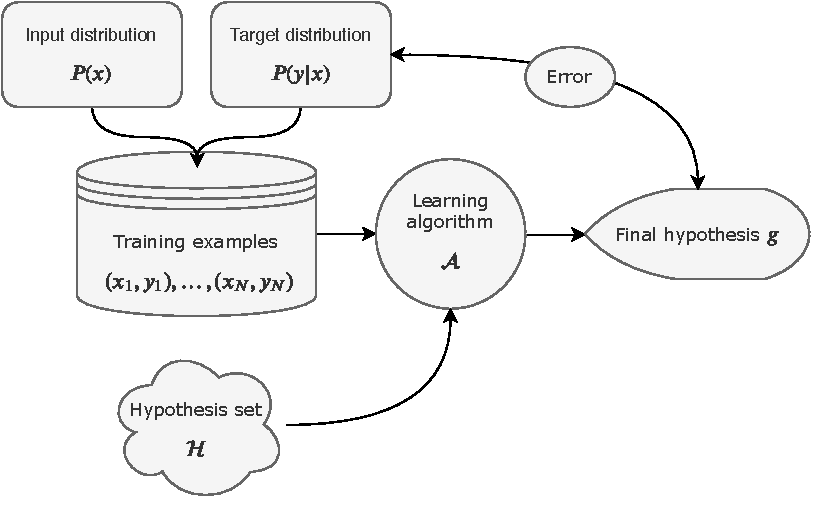
\includegraphics[width = \linewidth]{\imgpath/elements_learning.pdf}
  \end{center}
  \caption{Schematic of the main elements of (supervised) learning. Adapted from \citet{abu2012learningfromdata}.}
\label{fig:background-elements_learning}
\end{figure}

The feasibility of learning from a mathematical and probabilistic perspective is studied by the field of statistical learning theory \citep{vapnik1995learningtheory, bousquet2003learningtheory, vonluxburg2011learningtheory}. In the next section, we introduce the important concept of generalisation in machine learning and some notions from learning theory that are relevant to this thesis. 

\subsection{Theory of generalisation}
\label{sec:background-generalisation}
Generalisation is one of the most important concepts in machine learning and statistical learning theory. It refers to the idea that the ultimate goal in the learning process is not to minimise the error computed on the available training data in and of itself, but to perform well on unseen data, that is to generalise. This raises the reasonable first question of whether generalisation is possible at all. The probabilistic perspective not only provides a positive answer to the question but also the tools to analyse the generalisation guarantees of learning algorithms.

\subsubsection{Empirical risk minimisation}
In order to elaborate this idea, let us first introduce some important concepts that we will use in this section and throughout the thesis. To formally describe the problem at hand, we recall that we consider data that consist of the inputs $\mathbf{x}_{i} \in \mathcal{X}$ and the outputs or targets $y_{i} \in \mathcal{Y} = \{-1, 1\}$, that is binary classification, for simplicity of the exposition. Furthermore, we assume that the pairs $(\mathbf{x}_{i}, y_{i}) \in \mathcal{X} \times \mathcal{Y}$ are independently and identically sampled according to an unknown probability distribution $P_{X,Y}$. So as to measure the discrepancy between the target variables $y$ and the outcome of the hypotheses $h(x)$,\footnote{The hypotheses depend on both $\mathbf{x}$ and $\boldsymbol{\theta}$, that is $h(\mathbf{x}; \boldsymbol{\theta})$, but we will in general abuse notation and write simply $h(x)$, or even just $h$, for better readability.} we assume that we are given a real-valued \textit{loss function} $L(y, h(x))$. Since we are considering binary classification, the loss function will be the classification error: $L(y, h(x)) = \mathbbm{1}_{h(x) \neq y}$. Then, the \textit{risk} associated with a hypothesis $h$ is given by the expectation of the loss function, defined by the following \textit{risk functional}:
%
\begin{equation}
    R(h) = \mathbb{E} \left[ L(y, h(x)) \right] = \int L(y, h(x))dP_{X,Y}(x, y)
\end{equation}

Ultimately, the goal of a learning algorithm is to find the optimal hypothesis $h^{*} \in \mathcal{H}$ that minimises the risk $R(h)$:
%
\begin{equation}
    h^{*} = \argmin_{h \in \mathcal{H}} R(h)
\end{equation}

However, because the joint probability distribution $P_{X,Y}$ is unknown, it is not possible to exactly calculate $R(h)$. In practice, the risk functional is replaced by the computation of the \textit{empirical risk} on the set of $N$ available data points:
%
\begin{equation}
    R_{N}(h) = \frac{1}{N} \sum_{i=1}^{N} L(y_{i}, h(x_{i}, \theta))
\end{equation}
%
and the learning algorithm chooses the hypothesis $g$ by minimising the empirical risk:
%
\begin{equation}
    g = \hat{h} = \argmin_{h \in \mathcal{H}} R_{N}(h)
\end{equation}

This method is known as the \textit{Empirical Risk Minimisation} inductive principle (ERM) \cite{vapnik1982erm, vapnik1992erm}. The ERM principle was thoroughly studied during the 1960--1990s by Vladimir Vapnik and Alexey Chervonenkis, as well as other scientists, and it is summarised in the book \textit{The nature of statistical learning theory} \cite{vapnik1995learningtheory}. Empirical risk minimisation is a general principle and many classical estimation methods, such as least squares regression and maximum likelihood estimation, can be formulated as realisations of the ERM principle.

Some important aspects of the theory explained in the book and studied in a number of publications are the necessary and sufficient conditions for the consistency of algorithms based on the ERM, that is under what conditions minimising the empirical risk converges in the minimisation of the risk, when the number of examples tends to infinity \cite{vapnik1991necessary}; the rate of convergence of learning processes based on the ERM. Here, we will summarise the most important aspects and concepts of the learning theory based on the ERM.

\subsubsection{Uniform bounds}
Having outlined the notion of empirical risk minimisation and its components, we can define generalisation as the ability of a learning algorithm to achieve small risk $R(h)$. We can now return to the question of the feasibility of generalisation or the consistency of a learning process. An important result from probability theory that serves as starting point to study the feasibility of learning is Hoeffding's inequality \cite{hoeffding1963hoeffding}. It states that for any $\varepsilon > 0$ and a set of $N$ i.i.d. random variables $Z_{1} \ldots Z_{N}$, such that $\mathbb{P} \left[a \leq Z_{i} \leq b \right] \forall i$, then:
%
\begin{equation}
\label{eq:background-hoeffdings}
    \mathbb{P} \left[ \left| \frac{1}{N} \sum_{i=1}^{N}Z_{i} - \mathbb{E}\left[Z\right] \right| > \varepsilon \right] \leq 2 \exp \left( -\frac{2\varepsilon^{2}N}{(b-a)^{2}} \right)
\end{equation}

Hoeffding's inequality can be regarded as quantitative version of the law of large numbers\footnote{The law of large numbers is a fundamental theorem from probability theory. It states that the sample average converges in probability towards the expected value as the sample size increases.} for the case when the variables are bounded. Equation~\ref{eq:background-hoeffdings} can be developed into a more useful form for our purposes, relating the risk of a hypothesis, $R(h)$, and the empirical risk, $R_{N}(h)$. For any $\delta > 0$, at least with probability $1 - \delta$:
%
\begin{equation}
\label{eq:background-hoeffdings_risk_single}
    R(h) \leq R_{N}(h) + \sqrt{\frac{1}{2N}\log\frac{2}{\delta}}
\end{equation}

The interpretation of Equation~\ref{eq:background-hoeffdings_risk_single} is that the risk of hypothesis $h$ is bounded by a quantity that depends linearly and on the empirical risk plus a constant that depends on the number of samples used to obtain the empirical risk and the confidence $\delta$. On the one hand, this is good news as it establishes that the empirical risk is indicative of the true risk when the number of samples is large. This confirms the feasibility of learning. 

Nonetheless, on the other hand, the bound in Equation~\ref{eq:background-hoeffdings_risk_single} is highly limited and useless in practice. Essentially, it says that for each hypothesis $h$, there exists a set of samples for which the bound holds. However, the function which will be chosen by the learning algorithm is unknown before training it on the data set. For instance, there exists, as well, a function for which the empirical risk is not indicative of the true risk at all. In order to derive tighter, more useful bounds we need to take into account all the possible hypotheses $\mathcal{H}$ that the learning algorithm may choose. One of the best studied approaches is to consider \textit{uniform bounds}.

The idea is to find an upper bound of the \textit{supremum} of $R(h) - R_{N}(h)$, as that will clearly provide an upper bound on $R(g)$:
%
\begin{equation}
    R(g) - R_{N}(g) \leq \sup_{h \in \mathcal{H}} \left[ R(h) - R_{N}(h) \right]
\end{equation}

The simplest way is to consider the disjunction of all events $\abs{R(h_{m}) - R_{N}(h_{m})} > \varepsilon$ for a finite set of hypothesis $\mathcal{H}$ of size $M$ and $m = 1, \ldots, M$. Then, by applying the union bound\footnote{$\mathbb{P}(\bigcup_{I}A_{i}) \leq \mathbb{P}(\sum_{i}A_{i})$} to the application of Hoeffding's inequality (see Equation~\ref{eq:background-hoeffdings}) to the union of the difference of the risk and the empirical risk for all hypotheses, we get that
%
\begin{equation}
\label{eq:background-uniform_bounds}
\begin{split}
    \mathbb{P} \left[ \left| R(h) - R_{N}(h) \right| > \varepsilon \right]& \leq \sum_{m=1}^{M} \mathbb{P} \left[ \abs{R(h_{m}) - R_{N}(h_{m})} > \varepsilon \right]\\ 
                                                                            & \leq 2M \exp(-2\varepsilon^{2}N)
\end{split}
\end{equation}
%
and hence, equivalent to Equation~\ref{eq:background-hoeffdings_risk_single}, for $\delta > 0$,  with probability at least $1 - \delta$:
%
\begin{equation}
\label{eq:background-hoeffdings_risk_all}
    R(g) \leq R_{N}(g) + \sqrt{\frac{1}{2N}\log\frac{2M}{\delta}}
\end{equation}

This is finally a practical error bound that guarantees that the risk of the final hypothesis $g$ found via empirical risk minimisation will be bounded by the empirical risk measured on the training set, as long as the hypothesis set is finite, that is $\abs{\mathcal{H}} = M$. A subtler implication of Equation~\ref{eq:background-uniform_bounds}, besides the fact that it leads to Equation~\ref{eq:background-hoeffdings_risk_all}, is that $R(g) \geq R_{N}(g) - \varepsilon$ also holds. Hence, the ERM principle ensures that there are not much better hypotheses than $g$ in the set $\mathcal{H}$.

While the generalisation bound based on uniform deviations is a key result in statistical learning theory and it is theoretically relevant, it is only valid for learning algorithms that operate with finite hypothesis sets. For many machine learning algorithms, the hypothesis sets are infinitely large and additional theoretical results are necessary to describe their generalisation guarantees. Below we present some of the most important results.

\subsubsection{Vapnik-Chervonenkis theory}
When the hypothesis set $\mathcal{H}$ is uncountable and thus the right hand side of Equation~\ref{eq:background-hoeffdings_risk_all} is unbounded, a classical approach is to use the notion of \textit{growth function}, also known as \textit{shatter coefficient} or \textit{shattering number}. The growth function $m_{\mathcal{H}}(N)$ was introduced by \citet{vapnik1971vc} and it denotes the maximal \textit{effective} size of $\mathcal{H}$ on a set of $N$ examples, that is the maximum number of ways into which $N$ data points can be classified by the function class. Formally: 
%
\begin{equation}
\label{eq:background-growth_function}
    m_{\mathcal{H}}(N) = \sup_{x_1, \ldots, x_N \in \mathcal{X}}\left| (h(x_1), \ldots, h(x_N)) : h \in \mathcal{H} \right|
\end{equation}

For the case of binary classification that we are considering, the growth function $m_{\mathcal{H}}(N) \leq 2^N$. If the hypothesis set is capable of generating all possible dichotomies (binary labellings) of $x_1, \ldots, x_N$, then $\mathcal{H}$ is said to \textit{shatter} the data set. If no data set of size $k$ can be shattered by $\mathcal{H}$, then $k$ is said to be a \textit{break point} for $\mathcal{H}$. 

One important concept in statistical learning theory is the Vapnik-Chervonenkis dimension, known as \textit{VC dimension} for short. The VC dimension of a hypothesis set $\mathcal{H}$, denoted by $d_{VC}(\mathcal{H}$) or simply $d_{VC}$ is the largest $N$ such that $m_{\mathcal{H}}(N) = 2^N$, that is the largest data set size that the hypothesis can shatter. Hence, if $d_{VC}$ is the VC dimension of $\mathcal{H}$, then $k = d_{VC} + 1$ is a break point for the growth function.

It can be shown that if a hypothesis class $\mathcal{H}$ has finite VC dimension $d_{VC}$, then the growth function can be upper bounded by a polynomial:
%
\begin{equation}
\label{eq:background-sauer_lemma}
m_{\mathcal{H}}(N) \leq \sum_{i=0}^{d_{VC}}{\binom{N}{i}}
\end{equation}

This allows us to bound the risk of a hypothesis in terms of the empirical risk and the growth function, what is known as the \textit{VC generalisation bound}. For $\delta > 0$,  with probability at least $1 - \delta$:
%
\begin{equation}
\label{eq:background-vc_bound}
    R(g) \leq R_{N}(g) + \sqrt{\frac{8}{N}\log\left(\frac{4m_{\mathcal{H}}(2N)}{\delta}\right)}
\end{equation}

The VC generalisation bound is a key result in statistical learning theory as it establishes the feasibility of learning with infinite hypothesis sets: with enough data, all hypotheses in an infinite $\mathcal{H}$ with finite VC dimension will generalise from the empirical risk. The bound holds for all hypothesis sets, learning algorithms, input spaces, probability distributions and binary targets \citep{abu2012learningfromdata}. Such generality comes at the expense of being quite a loose bound to be used in practice.

One interpretation of the generalisation bound in Equation~\ref{eq:background-vc_bound} that we will use in this thesis is that the right hand side consists of two terms: the empirical risk and a term that is usually interpreted as a penalty for model complexity:
%
\begin{equation}
\label{eq:background-vc_model_complexity}
\Omega(N, \delta, \mathcal{H}) = \sqrt{\frac{8}{N}\log\left(\frac{4m_{\mathcal{H}}(2N)}{\delta}\right)} \leq \sqrt{\frac{8}{N}\log\left(\frac{4(2N)^{d_{VC}}}{\delta}\right)}
\end{equation}

$\Omega$ depends on the number of examples $N$, the confidence parameter $\delta$ and the hypothesis class $\mathcal{H}$. The bound gets tighter (better) as the number of examples increases, as the confidence constant $\delta$ increases and as the complexity of the hypothesis set decreases (lower $d_{VC}$). This form of the bound on the risk, $R(g) \leq R_{N}(g) + \Omega(N, \delta, \mathcal{H})$, is found in most methods to estimate the theoretical generalisation guarantees of learning algorithms.

\subsubsection{Rademacher complexity}
\label{sec:background-rademacher}
Given these limitations of the Vapnik-Chervonenkis theory and, in particular, of the VC dimension, other measures of complexity have been developed \citep{bartlett2002complexity}. One relatively recent, popular example is the \textit{Rademacher complexity}, which allows to define generalisation bounds that are not restricted to binary classification and hold for any class of real-valued functions. 

Let $\sigma_1, \ldots, \sigma_N$ be a set of independent random variables such that $P(\sigma_i = 1) = P(\sigma_i = -1) = \frac{1}{2}$. These are known as \textit{Rademacher variables}, hence the name of the complexity measure. As before, we consider a sample of $N$ independent data points $x_1, \ldots, x_N$ defined on $\mathcal{X}$. Now, instead of being restricted to binary classification, we let $\mathcal{F}$ be the class of real-valued functions $f \colon \mathcal{X} \mapsto \mathbb{R}$. Then, the \textit{empirical Rademacher complexity} of $\mathcal{F}$ with respect to the sample of size $N$ is defined as:
%
\begin{equation}
\label{eq:background-empirical_rademacher_complexity}
  \hat{\mathcal{R}}_{N}(\mathcal{F}) = \mathbb{E}_{\sigma} \left[ \underset{f \in \mathcal{F}}{\mathrm{sup}} \left| \frac{1}{N} \sum_{i=1}^{N} \sigma_{i}f(x_{i}) \right| \right]
\end{equation}
%
where $\mathbb{E}_{\sigma}$ denotes the expectation with respect to the Rademacher variables. The \textit{Rademacher complexity}, also found in the literature as \textit{Rademacher average}, is defined as the expectation of the empirical Rademacher complexity over all data sets of size $N$ on $\mathcal{X}$:
\begin{equation}
\label{eq:background-rademacher_complexity}
  \mathcal{R}_{N}(\mathcal{F}) = \mathbb{E} \left[ \hat{\mathcal{R}}_{N}(\mathcal{F}) \right]
\end{equation}

The interpretation of the Rademacher average as a complexity measure is intuitive: It is a measure of the ability of the function class $\mathcal{F}$ to fit random noise, introduced by the Rademacher variables $\sigma_i$. For a very large and complex $\mathcal{F}$, there will be a function $f$ that can fit the noise, making $\hat{\mathcal{R}}_{N}(\mathcal{F})$ larger. 

For the case of binary classification that we have considered so far, in which $\mathcal{H} \subseteq \{h \colon \mathcal{X} \mapsto \mathcal{Y} = \{-1, 1\}\}$, it can be easily shown that $\hat{\mathcal{R}}_{N}(\mathcal{H}) = \frac{1}{2}\hat{\mathcal{R}}_{N}(\mathcal{F})$, using the fact that $\sigma_i$ and $\sigma_i Y_i$ have the same distribution. Finally, we can use the Rademacher complexity to bound the risk of the final hypothesis. For $\delta > 0$,  with probability at least $1 - \delta$:
%
\begin{equation}
\label{eq:background-rademacher_risk}
    R(g) \leq R_{N}(g) + \hat{\mathcal{R}}_{N} + \sqrt{\frac{2\log\frac{2}{\delta}}{N}}
\end{equation}

\subsection{Regularisation}
\label{sec:background-regularisation}
In Section \ref{sec:background-generalisation}, we have seen that the goal of a machine learning algorithm is to find a hypothesis $h(\mathbf{x})$ that, given some data $\mathcal{D} = \{(\mathbf{x}_{i}, y_{i})\}_{i}^{N}$, minimises the risk functional $R(h)$, which in turn depends on a loss function $L(y, h(\mathbf{x}))$ chosen as a criterion for the optimisation problem. We have also seen that, since it is not possible to exactly calculate the risk, in practice we optimise the empirical risk $R_{N}(h)$, which is calculated on the available training data:
%
\begin{equation}
\label{eq:background-argmin_empirical_risk}
    g = \argmin_{h \in \mathcal{H}} R_{N}(h)
\end{equation}

This method is known as empirical risk minimisation (ERM), and in Section~\ref{sec:background-generalisation} we have summarised the theory that describes the convergence of the empirical risk to the actual risk of the model. Nonetheless, despite the importance of this theory to confirm the feasibility of learning, the bounds on the generalisation error are not always applicable in practice: they are quite loose, depend on hypothesis sets with finite VC dimension and, in general, the plain ERM principle is intended to deal with large sample sizes. In practice, learning algorithms rely on extensions of ERM, such as the principle of structural risk minimisation (SRM) \citep{vapnik1974srm}. A particular case of SRM is regularisation, a widely used technique in machine learning and one of its cornerstones \citep{poggio1990regularisation, girosi1995regularization}. In this section we review the fundamentals of regularisation and present some of its most common forms, which are relevant for this thesis.

The concept of regularisation of learning algorithms is closely related to the mathematical problem of approximating a function from sparse data, that is finding $f \in \mathcal{F}$ such that $Af = F$. \citet{hadamard1902illposed} demonstrated that under some general circumstances this is an ill-posed problem. That is, an arbitrarily small deviation $\varepsilon$ of $F$ ($F_{\varepsilon}$ instead of $F$, where $\norm{F - F_{\varepsilon}} < \varepsilon$) can cause large deviations in the solution of the equation. Formally, minimising the functional
%
\begin{equation}
\label{eq:background-ill_posed_functional}
    \rho(f) = \norm{Af - F_{\varepsilon}}^2
\end{equation}
%
is not guaranteed to provide a good approximation even if $\varepsilon$ tends to zero. This closely resembles the learning problem that we have described above, where the task is to find the function $g$ that best approximates the data $\mathcal{D}$, using the empirical risk, as summarised in Equation~\ref{eq:background-argmin_empirical_risk} and detailed in Section~\ref{sec:background-generalisation}. As a matter of fact, finding $g$ in the presence of noise is also ill-posed, as there is an infinite number of solutions. In order to find a suitable solution with access to only limited data, it is necessary to constrain the hypothesis space $\mathcal{H}$ with some a priori information, for instance assuming that the function is smooth. This is the idea of the regularisation principles discovered in the 1960s \citep{phillips1962regularisation, tikhonov1963regularisation, ivanov1976regularisation}. In particular, they found that if instead of minimising the functional $\rho(f)$ of Equation~\ref{eq:background-ill_posed_functional}, one minimises the so-called regularised functional
%
\begin{equation}
\label{eq:background-reg_functional}
    \rho^*(f) = \norm{Af - F_{\varepsilon}}^2 + \lambda(\varepsilon)\Omega(f)
\end{equation}
%
where $\Omega(f)$ is the regularisation functional, and $\lambda(\varepsilon)$ is a constant that determines the level of noise, then the sequence of solutions converges as $\varepsilon \rightarrow 0$. In our particular case of learning from data, the principles of regularisation translate into adding a similar regularisation term to the objective function. The similarity between the two problems is most obvious if we consider the mean squared error loss, instead of binary classification. In this case, the optimisation problem becomes the following:
%
\begin{equation}
\label{eq:background-reg_objective}
\begin{split}
	g &= \argmin_{h \in \mathcal{H}}R_{reg}(h) = \argmin_{h \in \mathcal{H}}\left[ R_{N}(h) + \lambda\Omega(h) \right]\\
      &= \argmin_{h \in \mathcal{H}}\left[ \sum_{i=1}^{N}(h(\mathbf{x}_{i}) - y_{i})^2 + \lambda\Omega(h) \right]
\end{split}
\end{equation}

$\Omega(h)$ is the regularisation functional or regulariser, which incorporates prior information or desired properties of the model. In general, the regulariser is chosen to encourage smooth functions. The constant $\lambda$ is the regularisation parameter, which controls the strength of the regularisation. 

The concepts of generalisation and particularly regularisation are closely related to the widely used concept of \textit{overfitting}, that is the tendency of a learning algorithm to excessively fit the training data points, to the detriment of its generalisation. Broadly speaking, a complex hypothesis function is more likely to \textit{overfit} the training data than a simpler function. The idea of function smoothness introduced by the regularisation term can be seen as a way to counteract overfitting, in favour of better generalisation. This establishes a trade-off where ideally the learning algorithm should strike the right balance between fitting the data, that is minimising the empirical risk, and finding a smooth enough function that generalises well. This trade-off can be controlled by the value of the regularisation parameter, which is often determined through \textit{cross-validation} \citep{stone1974crossval, allen1974crossval}. 

The choice of $\Omega(h)$ leads to different forms of regularisation and there is a very large body of literature on this topic. Popular choices are constraints on the norm of the parameters, which we will discuss in Section~\ref{sec:background-weight_decay} or constraints on the curvature of $h$. In modern machine learning, the concept of regularisation is very broad and regularisation is considered to be any mechanism that prevents overfitting, hence improving generalisation. In Chapter~\ref{ch:reg} we compare different forms of regularisation and discuss the distinction between implicit and explicit regularisation---key in Chapter~\ref{ch:daugreg}---and other regularisation taxonomies.

In the remaining of this section we introduce two specific regularisation techniques, weight decay and dropout, which are arguably the two most common forms of regularisation in modern neural networks.

\subsubsection{Weight decay}
\label{sec:background-weight_decay}
Weight decay is the common name used to refer to \textit{$L^2$--norm regularisation}\footnote{Note, however, that in part of the machine literature, the term weight decay refers to a form of regularisation in which the $L^2$--norm penalty is added directly to the update rule of gradient descent. This results in a conceptually equivalent form of regularisation, but with a slight numerical difference. See \citet{babenko2018wdvsl2} for more details.}, which is in turn a particular case of $L^p$--norm regularisation. In this section we will first review $L^p$--norm regularisation as a direct realisation of the type of regularisation described above, and then present the specific aspects of weight decay.

In the previous section we have seen that the concept of regularisation derived from the mathematical tool for solving ill-posed problems, results in a modification of the objective function (see Equation~\ref{eq:background-reg_objective}). We will denote the regularised objective by $\hat{J}$:
%
\begin{equation}
\label{eq:background-reg_objective_explicit}
    \hat{J}(\boldsymbol{\theta}; \mathbf{x}, y) = J(\boldsymbol{\theta}; \mathbf{x}, y) + \lambda\Omega(\boldsymbol{\theta})
\end{equation}

$L^p$--norm regularisation refers to the family of techniques which apply a penalty on the norm of the parameters:
%
\begin{equation}
\label{eq:background-l_p_norm}
\Omega(\boldsymbol{\theta}) = \phi(\norm{\boldsymbol{\theta}}_p) = \phi\left(\left(\sum_{i=1}^{d}\abs{\theta_i}^p\right)^{\frac{1}{p}}\right)
\end{equation}
%
where $\phi(\cdot)$ is an optional function applied on the norm, for example the squared function. The most commonly used $L^p$--norm penalties are $L^1$ and $L^2$ regularisation. $L^2$ regularisation is probably one of the most widely used regularisation techniques in machine learning. In deep learning, it is commonly referred to as \textit{weight decay}, but it is also known as Tikhonov regularisation \citep{tikhonov1963regularisation} or ridge regression when applied to linear regression. In this thesis, we will analyse weight decay in neural networks and compare it to other regularisation techniques in Chapter~\ref{ch:daugreg}, and we use it to regularise a logistic regression algorithm in Chapter~\ref{ch:globsal}.

The specific regularisation term typically used for weight decay is $\Omega(\boldsymbol{\theta}) = \frac{1}{2}\norm{\boldsymbol{\theta}}_2^2$ because it allows to implement and express the objective function in a convenient and efficient way using the dot product between the vector of parameters and its transpose:
%
\begin{equation}
\label{eq:background-weight_decay_objective}
    \hat{J}(\boldsymbol{\theta}; \mathbf{x}, y) = J(\boldsymbol{\theta}; \mathbf{x}, y) + \frac{\lambda}{2}\boldsymbol{\theta}^T\boldsymbol{\theta}
\end{equation}

Weight decay has been long used, at least since the 1980s \citep{hinton1987wd}, and widely studied, both empirically \citep{zhang2018wd} and theoretically \citep{krogh1992wd, neyshabur2015regularization}, especially in the context of neural networks. Intuitively, the mechanism provided by weight decay is to restrict the norm of the trainable parameters, by decreasing the weight vector at every iteration of a model trained with gradient descent, in the directions that do not contribute much to reducing the objective function. Relevant to this dissertation is the result by \citet{bishop1995tikhonov}, which showed that optimising a squared error loss with weight decay is equivalent to training with random noise in the inputs. In Chapter~\ref{ch:daugreg}, we will use this result to derive some theoretical insights into the comparison of weight decay and data augmentation.

\subsubsection{Dropout}
\label{sec:background-dropout}
Dropout is a regularisation technique first described by this name in \citep{hinton2012dropout, srivastava2014dropout}, although closely related to \textit{dilution} \citep{hertz1991dilution}. It is very widely used in modern neural networks due to its simplicity and effectiveness. In practice, dropout is implemented and hence can be described as a method that omits every unit---parameter, feature detector, etc.---of a model with probability $p$, at every iteration of the optimisation process (training). At inference (test) time, the whole set of units is considered. While dropout can be applied to a broad class of models, it is most often used to train deep neural networks and for simplicity we will also consider neural networks in this section.

Dropout is often described as a practical approximation of training an ensemble of models through bootstrap aggregation, commonly known as \textit{bagging} \citep{breiman1994bagging}, in which $M$ models are trained on $M$ subsets of a data set of size $N$ uniformly sampled with replacement (bootstrap sample). At inference time, the outputs of the $M$ models on each data point are averaged (for regression) or combined through majority voting (for classification). Bagging is a widely used technique, known to reduce the variance and overfitting of learning algorithms. However, it is computationally expensive as it requires training multiple models. Dropout efficiently approximates a form of bagging with an exponentially large number of sub-networks (models). Since neural networks are typically trained with mini-batch iterative methods (such as stochastic gradient descent), the parameters of the model are updated by computing the loss of a sub-network on a sub-sample of the data set. An important difference between standard bagging and dropout is that while in bagging the models are independent, with dropout the models share a subset of the parameters from the parent neural network.

In \citep{srivastava2014dropout}, dropout training is connected with a theory by \citet{livnat2010sex} about the superiority of sexual over asexual reproduction in nature. According to this theory, a criterion for natural selection would be enhancing the robust combination of different genes for better adaptation to changes, as opposed to the optimisation of the individual fitness through a slight mutation of one parent's genes. Sexual reproduction would favour this criterion by preventing co-adaptations of the available genes in one individual. With dropout, the units of a network are forced to learn useful combinations with other subsets of random units, hence preventing co-adaptation and increasing robustness.

Dropout has greatly impacted the deep learning community\footnote{The two original papers have been increasingly cited almost 25,000 times at the time of writing, according to Google Scholar.}. It is widely used for training neural networks in both research and application and it has been deeply studied both empirically and theoretically \citep{gal2016dropout}, sometimes uncovering contradictory and surprising properties. While it is out of the scope to review the vast literature on dropout training, we can mention some relevant findings. Since shortly after it was proposed, dropout has been analysed as adaptive form of regularisation \citep{wager2013dropout}. \citet{baldi2013dropout} found that the dynamics of gradient descent with dropout training approximate that of a regularised error function, while \citet{helmbold2017dropout} showed that in deeper networks, the behaviour of dropout differs significantly from standard regularisation. More recently, \citet{mou2018dropout} derived generalisation bounds based on the Rademacher complexity for deep neural networks trained with dropout. Finally, an interesting and relevant finding for this thesis is that dropout applied to the intermediate units of a neural network has been shown to be equivalent to training with noise in the input \citep{bouthillier2015dropoutasdaug}.

\chapterbibliography
}
